\section{Developed Control Software}\label{sec:software}
My thesis work was included in the development of \Qibolab~\cite{Efthymiou_2023}, the instrument-related component of the \Qibo~\cite{qibo-website} framework.

\begin{figure}[ht]
    \makebox[\textwidth][c]{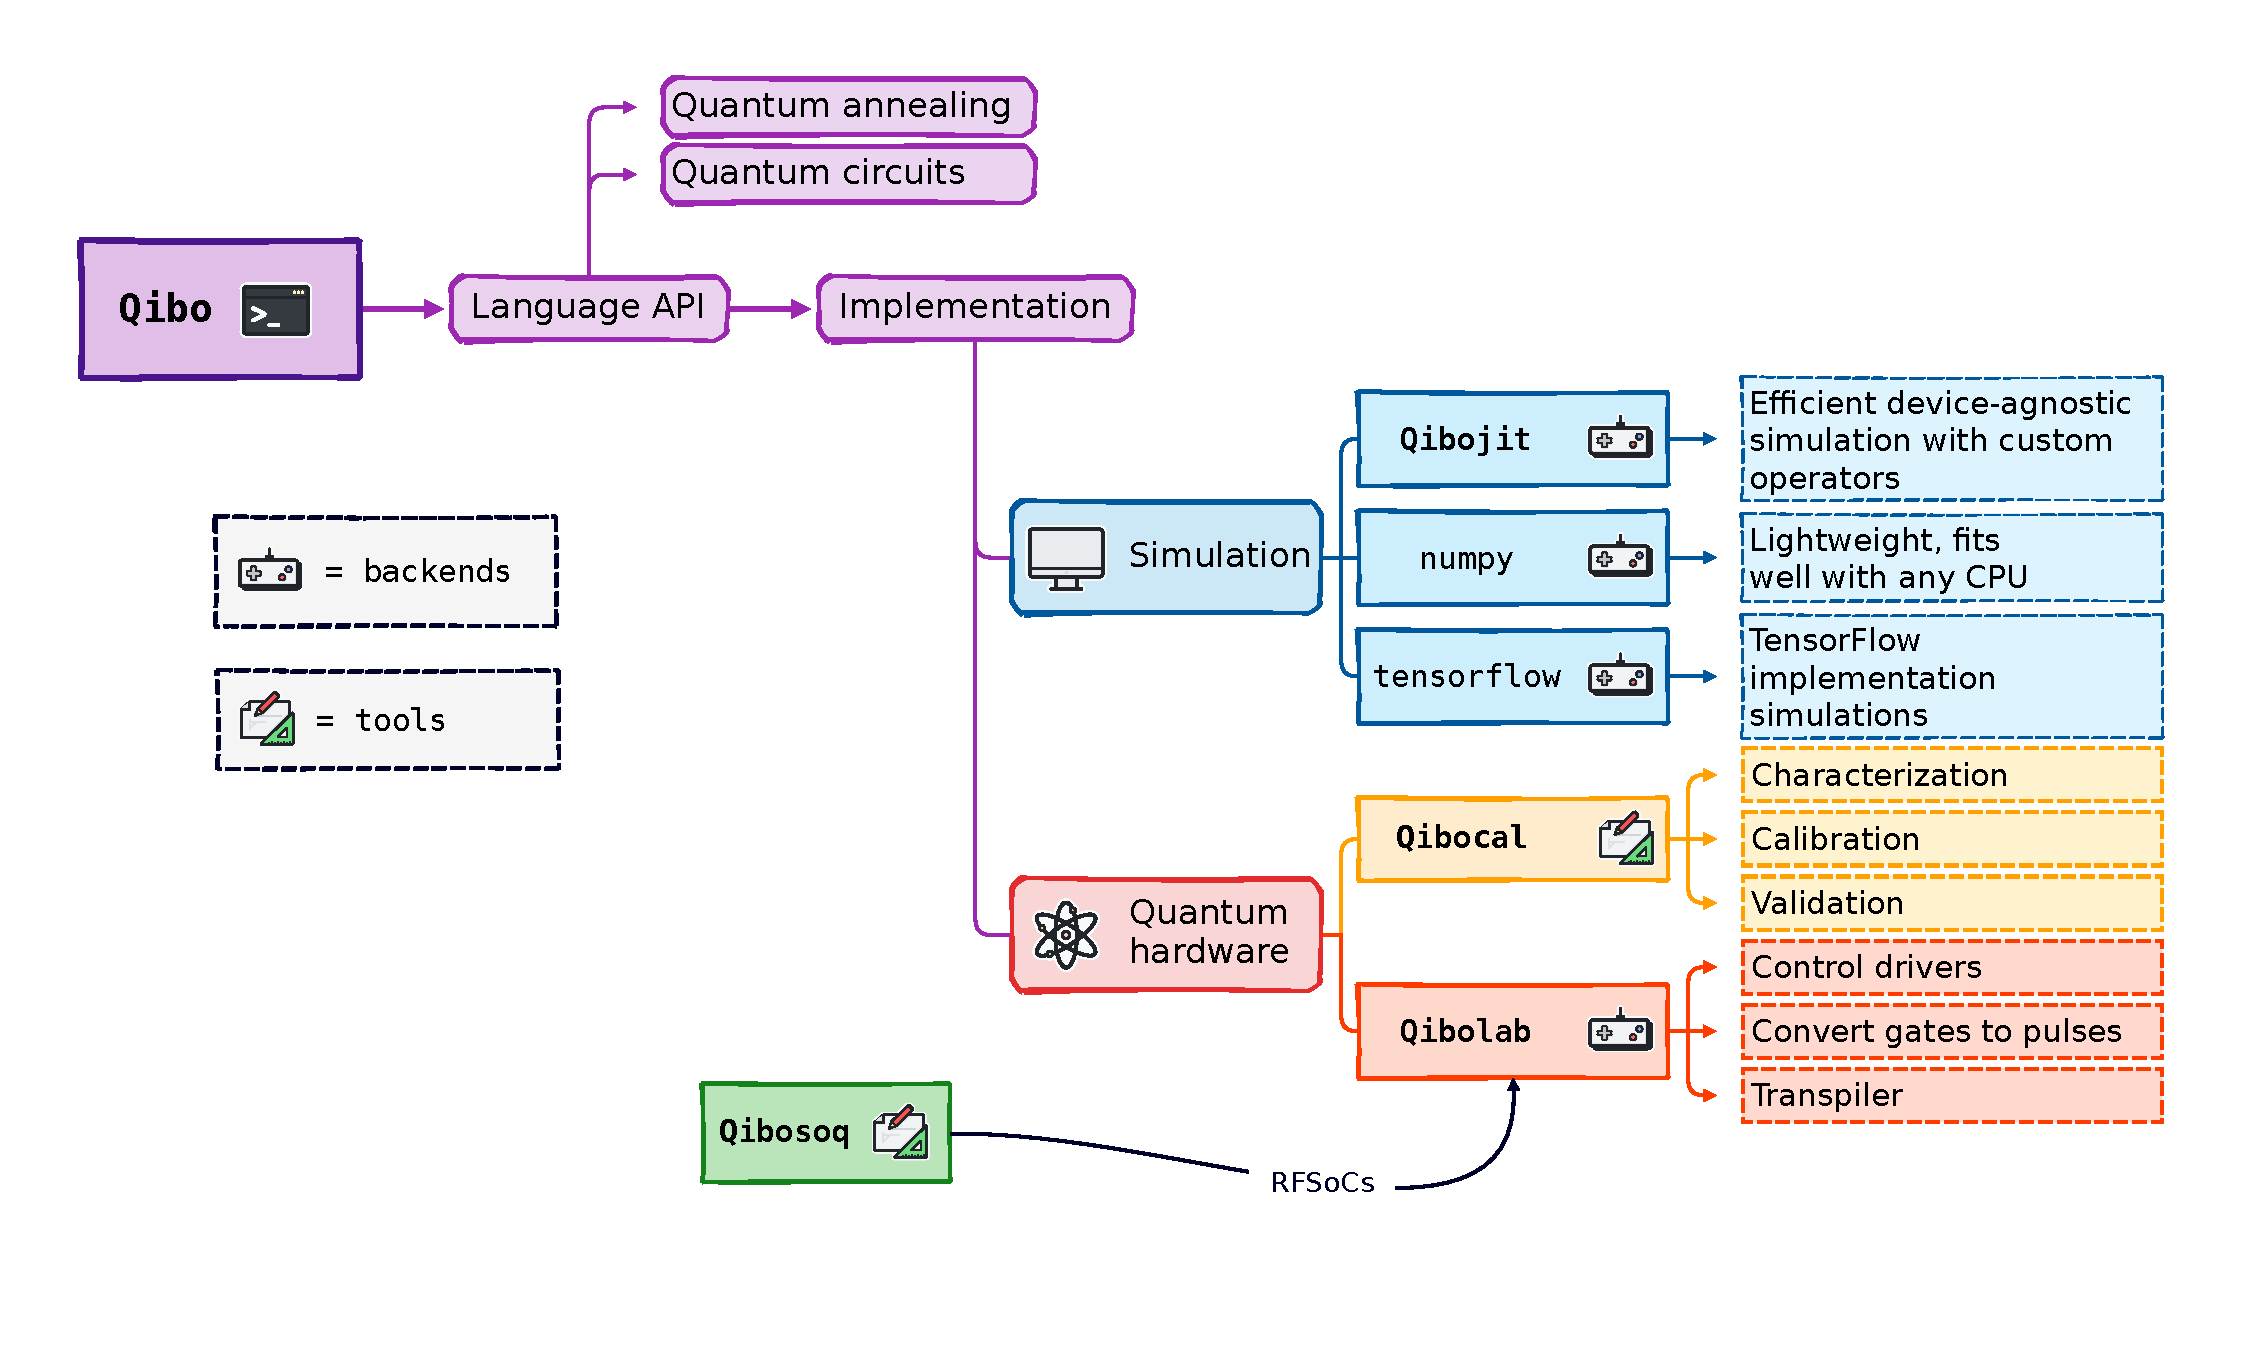
\includegraphics[width=1.3\textwidth]{Setup-software/figures/qibo_ecosystem.pdf}}
    \caption{Schematic overview of \Qibo software components.}
    \label{fig:qibo-ecosystem}
\end{figure}

\Qibo, schematically illustrated in \cref{fig:qibo-ecosystem}, is an open-source~\cite{qibo-github,qibolab-github,qibosoq-github} full stack application for quantum simulation that can be used to define and efficiently simulate circuits. 
It supports various backends for the execution of circuits: all of them are related to simulations, but one.

\Qibolab is the backend dedicated to hardware control and for deployment of circuits on real-quantum-hardware.
The idea behind \Qibolab is that of an hardware-agnostic software for hardware control that can be used in different laboratories without any development effort.\\
\Qibolab supports different control devices: in particular the systems of Quantum Machines, QBlox, Zurich-Instruments and, after my thesis, several RFSoC FPGAs.

In particular, I developed a two-side driver: composed of a client (the \Qibolab component) and a server called \Qibosoq.
The latter is a server that runs on the FPGA CPU present on the RFSoC boards and has the task of translating the programs received by \Qibolab (that are in the form of sequences of pulses) to a \Qick program.
\Qick contains both the firmware of the FPGAs and a low-level software to interact with the FPGA logic.

In this section I will give a general overview of the \Qibolab project, its components and abstraction levels and I will provide some details on the implementation of the RFSoC driver as well as of the \Qibosoq package. 

\subsection{Qibolab}

\Qibolab is the \Qibo backend dedicated to hardware execution.

Ideally, \Qibolab wants to be a universal control software for quantum computing, usable in the control of different qubit technologies by different electronics.
The philosophy that is guiding the development of this tool is the \textit{middleware} one, from RedHat.com:
\begin{quote}
    Middleware is software and cloud services that provide common services and capabilities to applications and help developers and operators build and deploy applications more efficiently. Middleware acts like the connective tissue between applications, data, and users.
\end{quote}

So that's the idea. In a moment in which, for quantum computing, no instrument is compatible with another one, where every technology and company implements a new programming language, where there is no convention between different constructors, \Qibolab wants to be the glue.

The key features of the API (Application Programming Interface, namely the software abstractions and functionalities), as it is now, are:
\begin{itemize}
    \item support for \Qibo circuits deployment on quantum hardware;
    \item support for different instruments for custom lab setups and easy integration of new drivers;
    \item support for different heterogeneous platforms (qubit systems);
    \item re-usability of calibration experiments via \Qibocal.
\end{itemize}

\Qibolab is a complex library and is currently composed of roughly $25000$ lines of Python code ($79000$ total lines including also documentation and tests), its main components are:

\begin{description}
    \item[Platform] this is the object that orchestrates different instruments in a laboratory, it describes a set of controlled qubits, controller device and any additional required device to coordinate;
    \item[Qubits] objects that contain characterization/calibration parameters, information about native calibrated gates and the connected channels;
    \item[Channels] physical wires in a laboratory that describe the setup and the connection among instruments and between the controller and the qubit;
    \item[Pulses] extensive API to work with pulses and pulse sequences. It includes support of various shapes;
    \item[Sweepers] these are objects crucial for experiments since they enable fast scans directly looping on FPGA logic;
    \item[Transpiler and Compiler] two components that, working together, are in charge of converting a circuit to a list of pulses (first as a circuit of native gates and then as a list of "native pulses");
    \item[Instruments] one  of the most important parts of \Qibolab, comprehensive support of different instruments under the same interface.
\end{description}

The main instruments, often called controllers, are shown in \cref{fig:qibolab_instruments}, while a list of supported features is available in \cref{tab:drivers-features}.

\begin{figure}[ht]
    \centering
    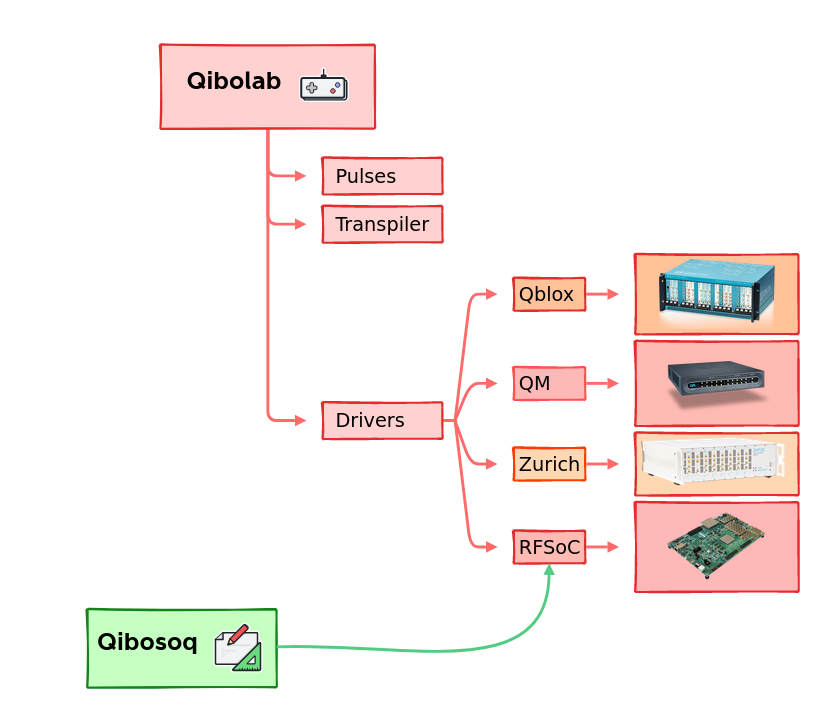
\includegraphics[width=0.8\textwidth]{Setup-software/figures/qibolab_instruments.png}
    \caption{Schematic overview of \Qibolab supported instruments.}
    \label{fig:qibolab_instruments}
\end{figure}

\begin{table}[ht]
\centering
	\begin{tabular}{lcccc}
  \hline \hline
		\textbf{Feature}              & \textbf{RFSoCs}    & \textbf{Qblox}    & \textbf{QM}        & \textbf{Zhinst}   \\ \hline
		Arbitrary pulse sequences     & \usym{1F5F8}  & \usym{1F5F8} & \usym{1F5F8}  & \usym{1F5F8} \\
		Arbitrary waveforms           & \usym{1F5F8}  & \usym{1F5F8} & \usym{1F5F8}  & ~\usym{1F5F8}\footnote{Sweeper capabilities may be reduced by using arbitrary pulses instead of driver defined ones.}      \\
		Multiplexed readout           & \usym{1F5F8}  & \usym{1F5F8} & \usym{1F5F8}  & \usym{1F5F8} \\
		Hardware classification       & \usym{2613}  & \usym{1F5F8} & \usym{1F5F8}  & \usym{1F5F8} \\
		Fast reset                    & \usym{1F4BB}   & \usym{1F4BB} & \usym{1F4BB}   & \usym{1F4BB}  \\
		Device simulation             & \usym{2613}  & \usym{2613} & \usym{1F5F8}  & \usym{1F4BB}  \\
		RTS frequency                 & ~\usym{1F5F8}\footnote{RTS on the frequency of readout pulses not supported.}    & \usym{1F5F8} & \usym{1F5F8}  & \usym{1F5F8}      \\
		RTS amplitude                 & \usym{1F5F8}  & \usym{1F5F8} & \usym{1F5F8}  & \usym{1F5F8} \\
		RTS duration                  & \usym{2613}  & \usym{1F5F8} & \usym{1F5F8}  & \usym{1F5F8} \\
		RTS start                     & \usym{1F5F8}  & \usym{1F5F8} & \usym{1F5F8}  & \usym{1F5F8} \\
		RTS relative phase            & \usym{1F5F8}  & \usym{1F5F8} & \usym{1F5F8}  & \usym{1F5F8} \\
		RTS 2D any combination        & \usym{1F5F8}  & \usym{1F5F8} & \usym{1F5F8}  & \usym{1F5F8} \\
		Sequence unrolling            & \usym{1F4BB}   & \usym{1F4BB} &\usym{1F4BB}  & \usym{1F4BB} \\
		Hardware averaging            & \usym{1F5F8}  & \usym{1F5F8} & \usym{1F5F8} & \usym{1F5F8} \\
		Singleshot (No Averaging)     & \usym{1F5F8}  & \usym{1F5F8} & \usym{1F5F8} & \usym{1F5F8} \\
		Integrated acquisition        & \usym{1F5F8}  & \usym{1F5F8} & \usym{1F5F8} & \usym{1F5F8} \\
		Classified acquisition        & \usym{1F5F8}  & \usym{1F5F8} & \usym{1F5F8}  & \usym{1F5F8} \\
		Raw waveform acquisition      & \usym{1F5F8}  & \usym{1F5F8} & \usym{1F5F8}  & \usym{1F5F8} \\
    \hline \hline
	\end{tabular}
	\caption[Supported features and limitations of \Qibolab \texttt{0.1.0}]{Features or limitations of the main drivers supported by \Qibolab \texttt{0.1.0}.
	The features denoted by `` \protect\usym{1F5F8} " are supported, `` \protect\usym{2613} "
  means not supported and `` \protect\usym{1F4BB} " under development.}
	\label{tab:drivers-features}
\end{table}

The following is a description of the features presented in \cref{tab:drivers-features}.
\begin{description}
    \item[Arbitrary pulse sequences] the capability of executing arbitrary pulse sequences defined in \Qibolab, which is a fundamental requirement of a driver. This feature is not related to the execution of pulses with arbitrary \textit{waveform shapes}.
    \item[Arbitrary waveforms] the capability of executing pulse waveforms of arbitrary shape. For drivers that do not support this feature, rectangular, Gaussian and Derivative Removal by Adiabatic Gate (DRAG~\cite{Gambetta2011}) waveforms can still be synthesized.
    \item[Multiplexed readout] allows playing and acquiring multiple multiplexed pulses through the same line. It is particularly useful for multi-qubit chips where the readout line is commonly shared among multiple qubits.
    \item[Hardware classification] the capability of doing single shot measurement classification \textit{during the execution} of a pulse sequence.
    \item[Fast reset] the capability of actively resetting the state of a qubit to zero after a measurement. This feature requires hardware classification and enables faster executions of repeated pulse sequences.
    \item[Device simulation] the possibility of simulating in advance the pulses to be executed, without directly using quantum hardware.
    \item[RTS frequency] RTS (\textit{Real Time Sweeper}) refers to the capability of executing a pulse sequence multiple times with different values of, in this case, the frequency of a pulse. This feature facilitates faster qubit characterization and experiments.
    \item[RTS amplitude] real-time sweeping of the amplitude of a pulse.
    \item[RTS duration] real-time sweeping of the duration of a pulse.
    \item[RTS start] real-time sweeping of the start time of a pulse.
    \item[RTS relative phase] real-time sweeping of the relative phase of a pulse.
    \item[RTS 2D] the capability of combining two RTS scans on different parameters.
    \item[Sequence unrolling] the capability of converting a sequence repeated multiple times, in a minor number of longer sequences that each contains multiple measurements, in order to decrease the overall time spent on pulse compilation and communication to the devices.
    \item[Hardware averaging] the capability of repeating the same experiment multiple times and obtain, directly from the device, averaged results.
    \item[Singleshot (No Averaging)] the capability of obtaining from the devices all the non-averaged results.
    \item[Integrated acquisition] the capability of acquiring complex signals~\cite{Naidu2003} with "in-phase" and "quadrature" (IQ) components demodulated and integrated for the measuring time.
    \item[Classified acquisition] the capability of performing 0-1 state classification after the integrated acquisition.
    \item[Raw waveform acquisition] the capability of acquiring non-integrated IQ waveform values.
\end{description}

\Qibolab was also object of a recent publication, in which the contribution of the work related to this thesis was not indifferent: CITE.


\subsection{Qibosoq}

A large part of my work for this thesis focused on the development of the required software to integrate RFSoCs into the \Qibo framework through \Qibolab driver.
To do so, it was needed to build a comprehensive library that bridged the differences between \Qibolab and \Qick (that has the task of controlling the FPGA logic).
This were the premises for \Qibosoq.

\Qibosoq is a an open-source server-side software package designed for RFSoC for executing arbitrary pulse sequences on self-hosted quantum processing units.

Its layout is essentially divided in three main elements:
\begin{description}
    \item[Client:] the user of the RFSoC, connected remotely via any network connection;
    \item[Server:] the always-listening server running directly on the board. It takes care of receiving commands from the client and to execute the experiments;
    \item[Language API:] a set of objects that define a common language between client and server.
\end{description}

The server role is to take commands and programs defined in the \Qibosoq language and compile them as an executable that can be run by the \Qick tProcessor: a timed processor on the FPGA logic that takes care of orchestrating firing pulses.

\Qibosoq exposes various tools and abstractions to the user: the \textbf{programs}, representing \Qick programs, and eventually taking care of the experiment compilation into the tProcessor language, the \textbf{components}, high-level structures used in the \textit{programs} construction, the \textbf{server} implementation, and \textbf{client} utilities, to manage the communication.

The \textbf{programs} bridge the gap between the high-level interfaces (components) and the low-level execution on quantum hardware.
Eventually, only two distinct programs are directly used, but the full hierarchy also includes intermediate abstractions.
Considering all layers, the defined \textbf{programs} are:
\begin{itemize}
    \item the abstract \textbf{base} program, that contains functions shared among all possible experiments and executions. It serves as the foundation for all the other \Qibosoq programs;
    \item the abstract \textbf{flux} program, that collects the additional elements required for controlling flux-tunable qubits. In addition to the functionalities defined in \textbf{base}, it includes support for bias voltages and fast DC (direct current) pulses.
    \item the \textbf{sequences} and \textbf{sweepers} programs, that contain the different elements used, respectively, in the execution of fixed parameters pulse sequences and real-time sweeps. They inherit all the functionalities defined in \textbf{base} and \textbf{flux}.
\end{itemize}

The \textbf{components} play the crucial role of establishing a common language for communication, easing the implementation of a \Qibosoq client in \Qibolab or by other parties.
The main elements defined within the \textbf{components} submodule include:
\begin{itemize}
    \item the \textbf{Config} object that contains essential general information required for execution on hardware, such as the number of repetitions for the experiment and the waiting time between repetitions;
    \item the \textbf{Pulse} base object that serves as the foundation for different implemented pulse shapes. Rectangular, Gaussian and DRAG~\cite{Gambetta2011} pulses are natively supported, as well as custom waveform shapes defined by their ''in-phase`` and ''quadrature`` (IQ)~\cite{Franks1969,Naidu2003} values;
    \item the \textbf{Qubit} object that describes a qubit and holds information about any necessary bias required for its operation~\cite{Hutchings2017};
    \item the \textbf{Sweeper} and \textbf{Parameter} objects that are used to describe real-time on-hardware scans.
\end{itemize}

\begin{table}[ht]
\centering
	\begin{tabular}{lccc}
  \hline \hline
		\textbf{Feature}  & \textbf{Qick} & \textbf{Qibolab} & \textbf{Qibosoq} \\ \hline
		Arbitrary pulse sequences     & \usym{1F5F8}  & \usym{1F5F8} & \usym{1F5F8}\\
		Arbitrary waveforms           & \usym{1F5F8}  & \usym{1F5F8} & \usym{1F5F8} \\
		Multiplex readout             & \usym{1F5F8}\footnote{Special firmware available from \Qick under request}  & \usym{1F5F8} & \usym{1F5F8} \\
		Feedback                      & \usym{1F5F8}  & \usym{1F5F8} & \usym{26ED} \\
		RTS frequency drive           & \usym{1F5F8} & \usym{1F5F8} & \usym{1F5F8}      \\
		RTS frequency readout         & \usym{2613}  & \usym{1F5F8} & \usym{2613}     \\
		RTS amplitude                 & \usym{1F5F8}  & \usym{1F5F8} & \usym{1F5F8} \\
		RTS duration                  & \usym{2613}  & \usym{1F5F8} & \usym{2613}  \\
		RTS start                     & \usym{1F5F8}  & \usym{1F5F8} & \usym{1F5F8}   \\
		RTS relative phase            & \usym{1F5F8}  & \usym{1F5F8} & \usym{1F5F8}   \\
		RTS N-Dimensional             & \usym{1F5F8}  & \usym{1F5F8} & \usym{1F5F8}   \\
		Hardware averaging            & \usym{1F5F8}  & \usym{1F5F8} & \usym{1F5F8}  \\
		Singleshot (No Averaging)     & \usym{1F5F8}  & \usym{1F5F8} & \usym{1F5F8}  \\
		Integrated acquisition        & \usym{1F5F8}  & \usym{1F5F8} & \usym{1F5F8}  \\
		Raw waveform acquisition      & \usym{1F5F8}  & \usym{1F5F8} & \usym{1F5F8}   \\
    \hline \hline
	\end{tabular}
	\caption[Comparison of the supported features of \Qibolab, \Qick and \Qibosoq]{Main features and limitations of \Qick, \Qibosoq and \Qibolab compared.
	The features denoted by `` \protect\usym{1F5F8} '' are supported, `` \protect\usym{2613} ''
    means not supported and `` \protect\usym{26ED} '' under development.}
	\label{tab:supported-features_qibosoq}
\end{table}


The last two fundamental elements are the \textbf{client} and the \textbf{server}.
The \textbf{client} is composed of a set of tools used to connect to the server, convert components into a serialized form, and send them following the \Qibosoq communication protocol.
The \textbf{server} implements the on-board server, continuously listening for connections, and executing received instructions by initializing and running the required programs on the quantum hardware.

In analogy of what was presented for \Qibolab, in \cref{tab:supported-features_qibosoq} are presented the main features supported by \Qibosoq in comparison with what is supported by \Qick and \Qibolab.


\Qibosoq was developed for this thesis and is now a small complete library of $2500$ lines of python code (total of $8000$ lines) has been recently object to arXiv publication:~\cite{qibosoq_paper}.
